% !Mode:: "TeX:UTF-8"
%!TEX program  = xelatex

%\documentclass{cumcmthesis}
\documentclass[withoutpreface,bwprint]{cumcmthesis} %去掉封面与编号页



\usepackage{url}
\title{小锅的机器学习笔记--数学基础}


\schoolname{苏州大学}


\begin{document}
	\makeatletter %使\section中的内容左对齐
	\renewcommand{\section}{\@startsection{section}{300}{0mm}
		{-\baselineskip}{0.5\baselineskip}{\bf\leftline}}
	\renewcommand{\subsection}{\@startsection{section}{300}{5mm}
		{-\baselineskip}{0.5\baselineskip}{\bf\leftline}}

	


 \maketitle

%目录
%\tableofcontents
%\newpage
\section{\Large 数据集}

	每一个样本都是一个$p$维向量,记为:
	\begin{equation}
		x_i=(x_{i1},x_{i2},\ldots,x_{ip})^T
	\end{equation}
	我们不妨假设收集到的数据集一共有$N$个样本点,那么数据集可用$X_{N{\times}p}$ 来表示,记为:
	\begin{equation}
		X_{N{\times}p} ={(x_1,x_2,\ldots,x_N)}^{T}=
		\left(
		\begin{array}{cccc}
			x_{11} & x_{12} & \ldots & x_{1p}\\
			x_{21} & x_{22} & \ldots & x_{2p}\\
			\vdots & \vdots & \ddots & \vdots\\
			x_{N1} & x_{N2} & \ldots & x_{Np}\\
		\end{array}
		\right)_{N{\times}p}
	\end{equation}
\section{\Large 频率派}
	
	我们认为$\theta$ 是一个未知的常量,而$X_{N{\times}p}$是一个随机变量。
	那么每一个观测都是由$p\left(x_i|{\theta}\right)$所产生的,假设样本之间相互独立,那么对于整个数据集的观测为:
	\begin{equation}
		p\left(
			X_{N{\times}p}|{\theta}
		\right)=\prod \limits_{i=1}^N{p\left(x_i|{\theta}\right)}
	\end{equation}
	为了求最合适的$\theta$,我们采用$MLE$(极大对数释然估计)的方法求解:
	\begin{equation}
		{\theta}_{MLE}={\mathop{argmax}\limits_{\theta}}\log\,{p\left(
			X_{N{\times}p}|{\,\theta}
			\right)}={\mathop{argmax}\limits_{\theta}} \sum_{i=1}^N \log\, {p\left(x_i|{\theta}\right)}
	\end{equation}
\section{\Large 贝叶斯派}
	贝叶斯认为:$\theta$ 不是一个常量,而是满足一个预设的先验分布$\theta ~ p(\theta)$,那么依赖观察集的后验可以写成是:
		\begin{equation}
			p(\theta|X)=\dfrac{p(\theta,X)}{p(X)}=\dfrac{p(X|\theta) {\times} p(\theta)}{p(X)}
		\end{equation}
	如果这个$p$可能是离散型的随机变量,或者是连续型的随机变量。

		\[
		p(X)=\begin{cases}
			\int p(X|\theta){\times}p(\theta) d{\theta}	& \text{if } \theta \text{是连续型的随机变量} \\
			 \sum_{i=0}^n p(X|{\theta}_{i}){\times}p(\theta_{i}) & \text{if }  \theta \text{是离散型的随机变量}
		\end{cases}	
		\]
	可以注意到分母$p(X)$和$\theta$没有关系,为了求最合适的$\theta$,最大化这个$p(\theta|X)$:
	\begin{equation}
		\theta_{MAP}={\mathop{argmax}\limits_{\theta}} \,p(\theta|X)={\mathop{argmax}\limits_{\theta}}\, p(X|\theta) {\times} p(\theta)
	\end{equation}


	
	
\section{\Large 高斯分布}
	\subsection*{Data 假设}
		\begin{equation}
			x_i=\left(
				\begin{array}{c}
					x_{11} \\x_{12} \\ \vdots \\ x_{1p}\\
				\end{array}
			\right)
		\end{equation}
		\par
		\begin{equation}
			X_{N{\times}p} ={(x_1,x_2,\ldots,x_N)}^{T}=
			\left(
			\begin{array}{cccc}
				x_{11} & x_{12} & \ldots & x_{1p}\\
				x_{21} & x_{22} & \ldots & x_{2p}\\
				\vdots & \vdots & \ddots & \vdots\\
				x_{N1} & x_{N2} & \ldots & x_{Np}\\
			\end{array}
			\right)_{N{\times}p}
		\end{equation}
		
	\subsection*{一维的高斯分布}
	设$p=1$且我们设$X$满足高斯分布$N(\mu,\sigma)$
	$X$的概率密度为为:
	\begin{equation}
		p(x)=\dfrac{1}{\sqrt{2\pi}\sigma} \exp{(-\dfrac{(x-\mu)^2}{2\sigma^2} )}
	\end{equation}
	最后利用极大释然估计$X$ 的分布$N(\mu,\sigma)$
	\begin{align*}
		\log {p(X)} & = \log\prod \limits_{i=0}^N{p\left(x_i|{\theta}\right)} \\
				 &= \sum_{i=1}^N \log \,{p\left(x_i|{\theta}\right)}\\
				 &=-\sum_{i=1}^N \log{\sqrt{2\pi}}+\log{\sigma}+\dfrac{{(x_i-\mu)}^2}{2\sigma^2}				 
	\end{align*}
	那么$\mu_{MLE}$为:
	\begin{align*}
		\mu_{MLE} & ={\mathop{argmax}\limits_{\mu}}\,{\log {p(X)}}\\
		&={\mathop{argmax}\limits_{\mu}}\,-\sum_{i=1}^N \,{(x_i-\mu)}^2 \\
		&={\mathop{argmin}\limits_{\mu}}\,\sum_{i=1}^N \,{(x_i-\mu)}^2
	\end{align*}
	因为:
	\begin{equation}
		\frac{\partial \sum_{i=1}^N \,{{(x_i-\mu)}^2}}{\partial \mu}=2 \sum_{i=1}^N \,{(u-x_i)}=0
	\end{equation}
	所以有:
	\begin{equation}
		\mu_{MLE}=\dfrac{1}{N} \sum_{i=1}^N{x_i}
	\end{equation}
	对于另外一个参数$\sigma$:
	\begin{align*}
		\sigma_{MLE}&= {\mathop{argmax}\limits_{\sigma}}\,{\log {p(X)}}\\
		&={\mathop{argmax}\limits_{\sigma}}\,-\sum_{i=1}^N(\log{\sigma}+\dfrac{{(x_i-\mu)}^2}{2\sigma^2})\\
		&={\mathop{argmin}\limits_{\sigma}}\,\sum_{i=1}^N(\log{\sigma}+\dfrac{{(x_i-\mu)}^2}{2\sigma^2})		
	\end{align*}
	因为:
	\begin{equation}
		\frac{\partial  \sum_{i=1}^N(\log{\sigma}+\dfrac{{(x_i-\mu)}^2}{2\sigma^2})}{\partial \sigma^2}=\sum_{i=1}^N \dfrac{1}{2\sigma^2}-\dfrac{{(x_i-\mu)}^2}{2\sigma^4}=0
	\end{equation}
	所以有:
	\begin{equation}
		\sigma^2_{MLE}=\dfrac{1}{N}\sum_{i=1}^N{(x_i-\mu)^2}
	\end{equation}
	求解$\theta$的分布时,我们是先计算出$\mu_{MLE}$然后利用$\mu_{MLE}$求解得到$\sigma_{MLE}^2$。
	\begin{equation}
		E[\mu_{MLE}]=E[\dfrac{1}{N} \sum_{i=1}^N{x_i}]=\dfrac{1}{N} \sum_{i=1}^N{E[x_i]}=\mu
	\end{equation}
	\begin{align*}
		E[\sigma_{MLE}^2] & =E[\dfrac{1}{N}\, \sum_{i=1}^N \, x_i^2] - \mu_{MLE}^2\\
		&=\dfrac{1}{N}E[\sum_{i=1}^N (x_i^2-\mu^2)]-E[\mu_{MLE}^2-\mu^2]\\
		&=\dfrac{1}{N}\sum_{i=1}^N( E[x_i^2]-E[x_i]^2)-(E[\mu_{MLE}^2]-\mu^2)  \quad\quad\\
		 \text{因为 : }\\&\mu=E[\mu_{MLE}]\\
		&=\dfrac{1}{N}\sum_{i=1}^N(E[x_i^2]-E[x_i]^2)-(E[\mu_{MLE}^2]-E[\mu_{MLE}]^2)\\
		&=\dfrac{1}{N} \sum_{i=1}^N Var[x_i]-Var[u_{MLE}]
	\end{align*}
	\begin{align*}
		\text{ 因为 :   } &\\
		& Var[u_{MLE}] = \dfrac{1}{N^2} \sum_{i=1}^{N}\, Var[x_i]=\dfrac{1}{N}\sigma^2 \\
		& Var[x_i]=\sigma^2\\
		\text{ 所以 :   }&\\
		&E[\sigma_{MLE}^2]=\sigma^2-\dfrac{1}{N}\sigma^2=\dfrac{N-1}{N}\sigma^2
	\end{align*}
	所以可以发现对$\mu_{MLE}$是无偏的,但是对$\sigma_{MLE}$的估计是有偏的,上述的点估计方法会把$\sigma$估计小,
	通常取:
	\begin{equation}
		\sigma=\dfrac{1}{N-1}\sum_{i=1}^{N}(x_i-\mu)^2
	\end{equation}
	来进行修正。
	\subsection*{多维的高斯分布}
	首先$x$是一个$p$维的随机变量:
	\begin{equation}
		x \quad \~{} \~{} \quad N(\mu,\sigma)\quad \quad \\
		\hookrightarrow \quad f(x)=\dfrac{1}{(2\pi)^{\frac{p}{2}}|\Sigma|^{\frac{1}{2}}}\exp[-\dfrac{1}{2} (x-\mu)^T\Sigma^{-1}(x-\mu))]
	\end{equation}
	其中$\mu$为:
	\begin{equation}
		\mu=(u_1,u_2,\ldots,u_p)^T
	\end{equation}
	$\Sigma$协方差矩阵,一般而言是半正定矩阵,这里我们只考虑正定矩阵:
	\begin{equation}
		\Sigma=\left(\begin{array}{cccc}
			\sigma_{11} & \sigma_{12} &\ldots & \sigma_{1p}\\
			\sigma_{21} & \sigma_{22} &\ldots & \sigma_{2p}\\
			\sigma_{31} & \sigma_{32} &\ldots & \sigma_{3p}\\
			\vdots & \vdots & \ddots & \vdots\\
			\sigma_{p1} & \sigma_{p2} &\ldots & \sigma_{pp}
		\end{array}
		\right)
	\end{equation}
	因为$\Sigma$==$\Sigma^T$,所以这个$\Sigma$ 一定可以奇异值分解(也就是相似对角化)。
	\begin{equation}
		\Sigma=U{\Lambda}U^T
	\end{equation}
	其中:
	\begin{align*}
		U=(u_1,u_2,u_3,......,u_p)_{p{\times}p} &\quad u_i\text{是 $p$ 维列向量} \quad \text{并且 : } UU^T=U^TU=E\\
		&\Lambda=diag(\lambda_1,\lambda_2,....,\lambda_p)
	\end{align*}
	所以有:
	\begin{align*}
		\Sigma =U{\lambda}U^T=&\left(u_1,u_2,...,u_p\right) \left( 
			\begin{array}{cccc}
				\lambda_1 & 0 & \ldots & 0\\
				0 & \lambda_2 &  \ldots & 0\\
				\vdots  & \vdots  &  \ddots & \vdots \\
				0 & 0 & 0 & \lambda_p
			\end{array}
		\right)\left( 
			\begin{array}{c}
				u_1^T\\
				u_2^T\\
				\vdots\\
				u_p^T\\
			\end{array}
		\right)\\
		&=\left( u_1\lambda_1,u_2\lambda_2,...,u_p\lambda_p\right) \left( 
		\begin{array}{c}
			u_1^T\\
			u_2^T\\
			\vdots\\
			u_p^T\\
		\end{array}
		\right)\\
		&=\sum_{i=1}^{p} u_i \lambda_i u_i^T
	\end{align*}
	所以:
	\begin{equation}
		\Sigma ^{-1}=(U{\lambda}U^T)^{-1}=U{\lambda}^{-1}U^T=\sum_{i=1}^{p} u_i \dfrac{1}{\lambda_i} u_i^T
	\end{equation}
	现在我们设:
	\begin{equation}
		\bigtriangleup=(x-\mu)^T\Sigma^{-1}(x-\mu)=\sum_{i=1}^{p}(x-\mu)^T u_i \dfrac{1}{\lambda_i}u_i^T(x-\mu)
	\end{equation}
	显然有:
	\begin{align*}
		(x-\mu)^T u_i&=u_i^T(x-\mu)
	\end{align*}
	令:
	\begin{equation}
		y_i=(x-\mu)^T u_i\\
	\end{equation}
	\begin{equation}
		Y=(y_1,y_2,.....,y_p)^T
	\end{equation}
	所以:
	\begin{equation}
		\bigtriangleup=\sum_{i=1}^{p} \dfrac{y_i^2}{\lambda_i}
	\end{equation}
	\newpage
	那么$x$和$Y$之间有什么关系呢?我们现在设$x$为$p$维空间的一组向量,那么这个$Y$就是对$x$做了一轮可逆线性变换得到的。
	假设$x$是二维向量,并且规定$\bigtriangleup=1$,那么$x$和$y$之间的关系就如下图一样,
	\begin{figure}[h]
		\centering
		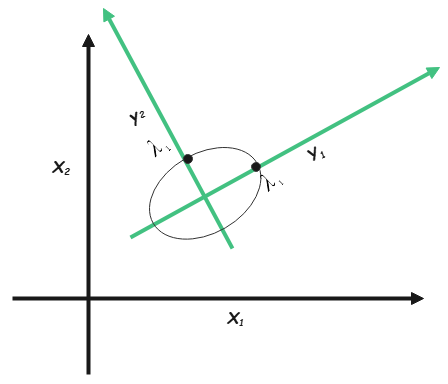
\includegraphics[width=10.0cm,height=8.0cm]{figures/x_y.png}
	\end{figure}
	也就是当$x$是一个二维向量时,固定$f(x)$的值,那么也等价于固定$\bigtriangleup$的值:
	\begin{equation}
		f(x)=Val
	\end{equation}
	所有满足$f(x)=Val$的二维向量$x$都在一个椭圆上,并且这个椭圆的圆心在向量$x$的坐标系中的坐标是均值向量$\mu$。
	当$p\geq3$,$x$是更高维度的向量时,所有满足$f(x)=Val$的二维向量$x$都在一个超椭球面上。
	\subsection{高斯分布-边缘概率和条件概率}
	设$x$ 是 两个随机变量$x_m,x_n$的联合随机分布:
	\begin{equation}
		x=\left(
			\begin{array}{c}
			x_1\\
			x_2\\
			x_3\\
			\vdots\\
			x_p 
		\end{array}
		\right)=\left( 
			\begin{array}{c}
				x_m\\
				x_n
			\end{array}
		\right)\quad \quad  \text{且满足 : }\quad m+n=p
	\end{equation}
	我们设:
	\begin{equation}
		\mu=\left(
		\begin{array}{c}
			\mu_1\\
			\mu_2\\
			\mu_3\\
			\vdots\\
			\mu_p 
		\end{array}
		\right)=\left( 
		\begin{array}{c}
			\mu_m\\
			\mu_n
		\end{array}
		\right)\quad \quad   \Sigma=\left( 
						\begin{array}{cccc}
							\sigma_{11} & \sigma_{12} & \ldots & \sigma_{1p} \\
							\sigma_{21} & \sigma_{22} & \ldots & \sigma_{2p} \\
							\vdots  & \vdots  &  \ddots & \vdots \\
							\sigma_{p1}& \sigma_{p2} & \ldots & \sigma_{pp}
						\end{array}
		\right)=\left( 
			\begin{array}{cc}
				\Sigma_{mm} & \Sigma_{mn}\\
				\Sigma_{nm}	& \Sigma_{nn}
			\end{array}
		\right)
	\end{equation}
	\textbf{然后我们引出一个推论:}\\
	已知随机变量 \quad$X \quad \~{} \~{} \quad N(\mu,\Sigma)$ ,并且$x\in R^p$,随机变量$Y=AX+B$,其中:矩阵$A_{q{\times}p}$,向量$B_{q}$,那么$Y$也服从高斯分布,且:
	\begin{equation}
		Y \quad \~{} \~{} \quad N(A\mu,A{\Sigma}A^T)
	\end{equation}
	\textbf{首先求解 $p(x_m)$:}
	我们设:
	\begin{equation}
		x_m=\left( 
			\begin{array}{cc}
				I_m & 0_n
			\end{array}
		\right)\left( \begin{array}{c}
				x_m\\
				x_n
		\end{array}
		\right)
	\end{equation}
	那么根据引出的推论:
	\begin{equation}
		A=\left( 
		\begin{array}{cc}
			I_m & 0_n
		\end{array}
		\right) \quad \quad B=0
	\end{equation}
	所以:
	\begin{equation}
		E[x_m]=\left( \begin{array}{cc}
			I_m & 0_n
		\end{array} \right) \left( 
		\begin{array}{c}
			\mu_m\\
			\mu_n
		\end{array}
	\right)=\mu_m
	\end{equation}
	\begin{equation}
		Var[x_m]=\left( \begin{array}{cc}
			I_m & 0_n
		\end{array} \right) \left( 
		\begin{array}{cc}
			\Sigma_{mm} & \Sigma_{mn}\\
			\Sigma_{nm} & \Sigma_{nn}
		\end{array}
		\right) \left( 
			\begin{array}{c}
				I_m\\
				0_n
			\end{array}
		\right)=\Sigma_{mm}
	\end{equation}
	所以我们知道(同理可求$x_n$):
	\begin{equation}
		x_m \quad \~{} \~{} \quad N(\mu_m,\Sigma_{mm})
	\end{equation}
	\textbf{然后求解 $p(x_n|x_m)$:}
		首先我们记:
		\begin{equation}
			x_{n.m}=x_n-\Sigma_{nm}\Sigma_{mm}^{-1}x_m=\left( 
				\begin{array}{cc}
					-\Sigma_{nm}\Sigma_{mm}^{-1} & I_n
				\end{array} 
			\right)
			\left( 
			\begin{array}{c}
				x_m\\
				x_n
			\end{array}
			\right)
		\end{equation}
	所以显然:
	\begin{equation}
		E[x_{n.m}]=\left( 
		\begin{array}{cc}
			-\Sigma_{nm}\Sigma_{mm}^{-1} & I_n
		\end{array} 
		\right) \left( 
			\begin{array}{c}
				\mu_{m}\\
				\mu_{n}
			\end{array}
		\right)=\mu_n-\Sigma_{nm}\Sigma_{mm}^{-1}\mu_m
	\end{equation}
	\begin{align}
		Var[x_{n.m}]&= \left( 
		\begin{array}{cc}
			-\Sigma_{nm}\Sigma_{mm}^{-1} & I_n
		\end{array} 
		\right) \left( 
			\begin{array}{cc}
				\Sigma_{mm} & \Sigma_{mn}\\
				\Sigma_{nm}	& \Sigma_{nn}
			\end{array}
		\right)\left( 
		\begin{array}{c}
			-\Sigma_{mm}^{-1}\Sigma_{nm}^{T} \\
			 I_n
		\end{array} 
		\right)\\&=
		\Sigma_{nn}-\Sigma_{nm}\Sigma_{mm}^{-1}\Sigma_{mn}
	\end{align}
	所以我们知道:
	\begin{equation}
		x_{n.m}  \quad \~{} \~{} \quad N(\mu_n-\Sigma_{nm}\Sigma_{mm}^{-1}\mu_m,\Sigma_{nn}-\Sigma_{nm}\Sigma_{mm}^{-1}\Sigma_{mn}) 
	\end{equation}
	可写成:
	\begin{equation}
		x_n=x_{n.m}+\Sigma_{nm}\Sigma_{mm}^{-1}x_m
	\end{equation}
	我们设随机变量$Z=x_n|x_m$,其实这个时候$x_m$是一个常量,那么本质上就是:
	\begin{equation}
		Z=x_{n.m}+\Sigma_{nm}\Sigma_{mm}^{-1}x_m \quad x_m\text{ 当做常量}
	\end{equation}
	借助引出的推论可知:
	\begin{equation}
		E[Z]=E[x_{n.m}]+ \Sigma_{nm}\Sigma_{mm}^{-1}x_m=\mu_n+\Sigma_{nm}\Sigma_{mm}^{-1}(x_m-u_m)
	\end{equation}
	\begin{equation}
		Var[Z]=Var[x_{n.m}]=\Sigma_{nn}-\Sigma_{nm}\Sigma_{mm}^{-1}\Sigma_{mn}
	\end{equation}
	所以我们知道了(同理可求$x_m|x_n$):
	\begin{equation}
		  x_n|x_m \quad \~{} \~{} \quad N(\mu_n+\Sigma_{nm}\Sigma_{mm}^{-1}(x_m-u_m),\Sigma_{nn}-\Sigma_{nm}\Sigma_{mm}^{-1}\Sigma_{mn}) \label{con:inventoryflow}
	\end{equation}
	\subsection*{高斯线性模型的求解}
	已知$x\quad \~{}\~{} \quad N(\mu,\Lambda^{-1})$,且$y|x \quad \~{} \~{} \quad N(Ax+b,L^{-1})$,求$y$和$x|y$的分布。\\
	首先计算$y$的分布,因为:\\$y|x \quad \~{} \~{} \quad N(Ax+b,L^{-1})$,这句话的意思是当$x$ 作为一个常量的时候,$y$服从一个均值为$Ax+b$,方差为$L^{-1}$的高斯分布,且$y$与$x$之间存在某种线性关系,所以我们设:。
	\begin{equation}
		y=Ax+b+\epsilon 
	\end{equation}
	\begin{align*}
	\text{且}&\quad\epsilon \quad\text{满足:} \quad  \epsilon \quad \~{} \~{} \quad N(0,L^{-1})
	\\ &\text{并且} \quad \epsilon \quad \text{与}\quad x \quad\text{相互独立} 
	\end{align*}
	根据引出的推论我们可以知道:
	 \begin{align*}
		E[y]&=E[Ax+b+\epsilon]=E[Ax+b]+E[\epsilon]\\
		&=A\mu+b
		\\Var[y]&=Var[Ax+b+\epsilon]=Var[Ax+b]+Var[\epsilon]\\
		&=A\Lambda^{-1}A^{T}+L^{-1}
	\end{align*}
	所以:
	\begin{equation}
		y \quad \~{} \~{}\quad N(A\mu+b,A\Lambda^{-1}A^{T}+L^{-1})
	\end{equation}
	下面求解$x|y$的分布,首先记:
	\begin{equation}
		Z=\left(
			\begin{array}{c}
				y\\
				x
			\end{array}
		 \right)
	\end{equation}
	很显然$Z$就是$x,y$的联合分布,$Z$的均值和方差为:
	\begin{equation}
		Z \quad \~{} \~{} \quad N(
		\left[
		\begin{array}{c}
			A\mu+b\\
			\mu
		\end{array}
		\right],\left[
			\begin{array}{cc}
				A\Lambda^{-1}A^{T}+L^{-1} &  Cov(y,x)\\
				Cov(x,y) &  \Lambda^{-1}
			\end{array}
		\right]
		) 
	\end{equation}
	下面求解$Cov(x,y)$:
	\begin{align*}
		Cov(x,y)&=E[(x-E[x])(y-E[y])^T]=E[(x-E[x])(Ax+b+\epsilon-E[Ax+b+\epsilon])^T]\\
		&=E[(x-E[x])(Ax-A\mu+\epsilon)^T]=E[(x-\mu)(x-\mu)^TA^T]+E[(x-\mu)\epsilon^T]
	\end{align*}
	我们知道$x$与$\epsilon$相互独立,所以$x-\mu$与$\epsilon$ 相互独立,所以有:
	\begin{equation}
		E[(x-\mu)\epsilon^T]=E[(x-\mu)]E[\epsilon^T]=0
	\end{equation}
	对于$E[(x-\mu)(x-\mu)^TA^T]$,有:
	\begin{equation}
		E[(x-\mu)(x-\mu)^TA^T]=E[(x-\mu)(x-\mu)^T]A^T =Var(x)A^T=\Lambda^{-1}A^T
	\end{equation}
	所以有:
	\begin{equation}
		Cov(x,y)=\Lambda^{-1}A^T
	\end{equation}
	并且:
	\begin{equation}
		Cov(y,x)=Cov(x,y)^T=A\Lambda^{-1}
	\end{equation}
	由公式(\ref{con:inventoryflow})我们可以知道:
		\begin{equation}
			E[x|y]=\mu+\Lambda^{-1}A^T(A\Lambda^{-1}A^T+L^{-1})^{-1}(y-A\mu-b)
		\end{equation}
		\begin{equation}
			Var[x|y]=\Lambda^{-1}-\Lambda^{-1}A^T(L^{-1}+A\Lambda^{-1}A^{T})^{-1}A\Lambda^{-1}
		\end{equation}
	所以:
	\begin{equation}
			x|y \quad \~{} \~{}\quad N(E[x|y],Var[x|y])
	\end{equation}
	\section{\Large 矩阵求导 }
	\subsection{分子布局与分母布局:}
	第一种情况,设:
	\begin{equation*}
		y \in R  \quad \quad x=\left( 
			\begin{array}{c}
				x_1\\
				x_2\\
				
				\vdots
				x_m
			\end{array}
		\right) \quad \quad x \in R_{m\times1}
	\end{equation*}
	也就是$y$是一个标量,$x$是一个m维的列向量,求$\dfrac{\mathrm{d} y}{\mathrm{d} x}$:
	\begin{equation}
		=\begin{cases}
			\quad \left[ 
			\dfrac{\mathrm{d} y}{\mathrm{d} x_1}
			,\ldots,\dfrac{\mathrm{d} y}{\mathrm{d} x_m}
			\right]	& \text{ }  \text{分子布局}
			 \\
			\\
			\quad \left[ 
			\dfrac{\mathrm{d} y}{\mathrm{d} x_1}
			,\ldots,\dfrac{\mathrm{d} y}{\mathrm{d} x_m}
			\right]^T &	 \text{ }  \text{分母布局}
		\end{cases}	
	\end{equation}

第二种情况,设:
\begin{equation*}
	x \in R  \quad \quad y=\left( 
	\begin{array}{c}
		y_1\\
		y_2\\
		
		\vdots
		y_m
	\end{array}
	\right) \quad \quad y \in R_{m\times1}
\end{equation*}
也就是$x$是一个标量,$y$是一个m维的列向量,求$\dfrac{\mathrm{d} y}{\mathrm{d} x}$:
\begin{equation}
	\dfrac{\mathrm{d} y}{\mathrm{d} x}=\begin{cases}
		\quad \left[ 
		\dfrac{\mathrm{d} y_1}{\mathrm{d} x}
		,\ldots,\dfrac{\mathrm{d} y_m}{\mathrm{d} x}
		\right]^T	& \text{ }  \text{分子布局} 
		\\
		\\
		\quad \left[ 
		\dfrac{\mathrm{d} y_1}{\mathrm{d} x}
		,\ldots,\dfrac{\mathrm{d} y_m}{\mathrm{d} x}
		\right] &	 \text{ }  \text{分母布局}
	\end{cases}	
\end{equation}
就如上所述的那样,其实分子分母布局的区别就是:如果求导之后得到的向量的行数与分子的行数相等就是分子布局,如果和分母的行数相等就是分母布局。
	然后扩展到向量对向量求导中,设:
	\begin{equation}
		y=\left(
			\begin{array}{c}
				y_1\\
				y_2\\
				\vdots\\
				y_n
			\end{array}
		\right)_{n\times1} \quad \quad 
		x=\left( 
				\begin{array}{c}
				x_1\\
				x_2\\
				\vdots\\
				x_m
			\end{array}
		\right)_{m\times1}
	\end{equation}求$\dfrac{\mathrm{d} y}{\mathrm{d} x}$:

	
	\begin{equation}
		\text{分子布局:} \quad \quad \dfrac{\mathrm{d} y}{\mathrm{d} x}=\left[
		\begin{array}{c}
			\dfrac{\mathrm{d} y_1}{\mathrm{d} x}\\\\
			\dfrac{\mathrm{d} y_2}{\mathrm{d} x}\\
			\vdots \\
			\dfrac{\mathrm{d} y_n}{\mathrm{d} x}
		\end{array}
		\right] =\left[
		\begin{array}{cccc}
			\dfrac{\mathrm{d} y_1}{\mathrm{d} x_1} & \dfrac{\mathrm{d} y_1}{\mathrm{d} x_2}&\ldots & \dfrac{\mathrm{d} y_1}{\mathrm{d} x_m}\\\\
			\dfrac{\mathrm{d} y_2}{\mathrm{d} x_1} & \dfrac{\mathrm{d} y_2}{\mathrm{d} x_2}&\ldots & \dfrac{\mathrm{d} y_2}{\mathrm{d} x_m}\\\\
			\vdots & \vdots & \ddots & \vdots \\\\
			\dfrac{\mathrm{d} y_n}{\mathrm{d} x_1} & \dfrac{\mathrm{d} y_n}{\mathrm{d} x_2}&\ldots & \dfrac{\mathrm{d} y_n}{\mathrm{d} x_m}
		\end{array}
		\right]_{n{\times}m} 
	\end{equation}
	向量对向量求导得到的结果是一个矩阵,分子布局就是求导得到的矩阵行数和分子一样,列拉伸到与分母一样。
	\begin{equation}
		\text{分母布局:} \quad \quad \dfrac{\mathrm{d} y}{\mathrm{d} x}=\left[
		\begin{array}{c}
			\dfrac{\mathrm{d} y}{\mathrm{d} x_1}\\\\
			\dfrac{\mathrm{d} y}{\mathrm{d} x_2}\\\\
			\vdots \\\\
			\dfrac{\mathrm{d} y}{\mathrm{d} x_m}
		\end{array}
		\right] =\left[
		\begin{array}{cccc}
			\dfrac{\mathrm{d} y_1}{\mathrm{d} x_1} & \dfrac{\mathrm{d} y_2}{\mathrm{d} x_1}&\ldots & \dfrac{\mathrm{d} y_n}{\mathrm{d} x_1}\\\\
			\dfrac{\mathrm{d} y_1}{\mathrm{d} x_2} & \dfrac{\mathrm{d} y_2}{\mathrm{d} x_2}&\ldots & \dfrac{\mathrm{d} y_n}{\mathrm{d} x_2}\\\\
			\vdots & \vdots & \ddots & \vdots \\\\
			\dfrac{\mathrm{d} y_1}{\mathrm{d} x_m} & \dfrac{\mathrm{d} y_2}{\mathrm{d} x_m}&\ldots & \dfrac{\mathrm{d} y_m}{\mathrm{d} x_m}
		\end{array}
		\right]_{m{\times}n}
	\end{equation} 
	分子布局就是求导得到的矩阵行数和分母一样,行拉伸到与分母一样。\\
	\textbf{下面的讨论全部基于分母布局:}\\
	\textbf{二阶导数:}
	\begin{equation*}
		\text{设:}
		\quad x=\left[
			\begin{array}{c}
				x_1\\
				x_2\\
				\vdots\\
				x_m
			\end{array}
		\right]_{m{\times}1}  \quad \text{,} \quad
			f(x) \in R \quad \quad  \text{求:}\quad \dfrac{\mathrm{d}^2 f(x)}{\mathrm{d} x^2}
	\end{equation*}
	解,记:
	\begin{equation*}
		 \quad g=\dfrac{\mathrm{d} f(x)}{\mathrm{d} x}=\left[
			\begin{array}{c}
				\dfrac{\mathrm{d} f(x)}{\mathrm{d} x_1}\\\\
				\dfrac{\mathrm{d} f(x)}{\mathrm{d} x_2}\\\\
				\vdots\\\\
				\dfrac{\mathrm{d} f(x)}{\mathrm{d} x_m}
			\end{array}
		\right]
	\end{equation*}
	所以:\begin{equation}
		\dfrac{\mathrm{d}^2 f(x)}{\mathrm{d} x^2}=\dfrac{\mathrm{d} g}{\mathrm{d} x}=\left[
		\begin{array}{c}
			\dfrac{\mathrm{d} g}{\mathrm{d} x_1}\\\\
			\dfrac{\mathrm{d} g}{\mathrm{d} x_2}\\\\
			\vdots\\\\
			\dfrac{\mathrm{d} g}{\mathrm{d} x_m}
		\end{array}
		\right]=\left[
			\begin{array}{cccc}
				\dfrac{{\partial}^2 f(x)}{{\partial} x_1 \partial x_1} & \dfrac{{\partial}^2 f(x)}{{\partial} x_2 \partial x_1} & \ldots & \dfrac{{\partial}^2 f(x)}{{\partial} x_m \partial x_1}\\\\
				\dfrac{{\partial}^2 f(x)}{{\partial} x_1 \partial x_2} & \dfrac{{\partial}^2 f(x)}{{\partial} x_2 \partial x_2} & \ldots & \dfrac{{\partial}^2 f(x)}{{\partial} x_m \partial x_2}\\\\
				\vdots & \vdots & \ddots & \vdots \\\\
				\dfrac{{\partial}^2 f(x)}{{\partial} x_1 \partial x_m} & \dfrac{{\partial}^2 f(x)}{{\partial} x_2 \partial x_m} & \ldots & \dfrac{{\partial}^2 f(x)}{{\partial} x_m \partial x_m}
			\end{array}				
		\right]
	\end{equation}
	上述二次求导过程和高数里面学的求导过程类似,只不过利用到了布局知识。
	\subsection*{复核求导}
		加法:
		\begin{equation}
			x=\left[
				\begin{array}{c}
					x_1\\
					x_2\\
					\vdots\\
					x_m
				\end{array}
			\right] \in R^{m{\times}1} 
			\quad  y=f(x)=\left[
			\begin{array}{c}
				y_1\\
				y_2\\
				\vdots\\
				y_n
			\end{array}
			\right]  \in R^{n{\times}1} 
			\quad   z=g(x)=\left[
			\begin{array}{c}
				z_1\\
				z_2\\
				\vdots\\
				z_n
			\end{array}
			\right] \in R^{n{\times}1}
		\end{equation}
	求$\dfrac{\mathrm{d} (y+z)}{\mathrm{d} x}$:
	\begin{align*}
		\dfrac{\mathrm{d} (y+z)}{\mathrm{d} x}&=\dfrac{\mathrm{d} y}{\mathrm{d} x}+\dfrac{\mathrm{d} z}{\mathrm{d} x}
		=\left[
			\begin{array}{c}
				\dfrac{\mathrm{d} y}{\mathrm{d} x_1}\\\\
				\dfrac{\mathrm{d} y}{\mathrm{d} x_2}\\\\
				\vdots\\\\
				\dfrac{\mathrm{d} y}{\mathrm{d} x_m}
			\end{array}
		\right]_{m{\times}1}+\quad \left[
		\begin{array}{c}
			\dfrac{\mathrm{d} z}{\mathrm{d} x_1}\\\\
			\dfrac{\mathrm{d} z}{\mathrm{d} x_2}\\\\
			\vdots\\\\
			\dfrac{\mathrm{d} z}{\mathrm{d} x_m}
		\end{array}
		\right]_{m{\times}1}\\\\
		&=\left[
		\begin{array}{cccc}
			\dfrac{\mathrm{d} y_1}{\mathrm{d} x_1} & \dfrac{\mathrm{d} y_2}{\mathrm{d} x_1} & \ldots & \dfrac{\mathrm{d} y_n}{\mathrm{d} x_1} \\\\
			\dfrac{\mathrm{d} y_1}{\mathrm{d} x_2} & \dfrac{\mathrm{d} y_2}{\mathrm{d} x_2} & \ldots & \dfrac{\mathrm{d} y_n}{\mathrm{d} x_2} \\\\
			\vdots & \vdots & \ddots &\vdots\\\\
			\dfrac{\mathrm{d} y_1}{\mathrm{d} x_m} & \dfrac{\mathrm{d} y_2}{\mathrm{d} x_m} & \ldots & \dfrac{\mathrm{d} y_n}{\mathrm{d} x_m} 
		\end{array}
		\right]_{m{\times}n}+\quad \left[
		\begin{array}{cccc}
			\dfrac{\mathrm{d} z_1}{\mathrm{d} x_1} & \dfrac{\mathrm{d} z_2}{\mathrm{d} x_1} & \ldots & \dfrac{\mathrm{d} z_n}{\mathrm{d} x_1} \\\\
			\dfrac{\mathrm{d} z_1}{\mathrm{d} x_2} & \dfrac{\mathrm{d} z_2}{\mathrm{d} x_2} & \ldots & \dfrac{\mathrm{d} z_n}{\mathrm{d} x_2} \\\\
			\vdots & \vdots & \ddots &\vdots\\\\
			\dfrac{\mathrm{d} z_1}{\mathrm{d} x_m} & \dfrac{\mathrm{d} z_2}{\mathrm{d} x_m} & \ldots & \dfrac{\mathrm{d} z_n}{\mathrm{d} x_m} 
		\end{array}
		\right]_{m{\times}n}
	\end{align*}
	乘法:
	设:\begin{equation*}
		x=\left[
			\begin{array}{c}
			x_1\\
			x_2\\
			\vdots\\
			x_m
		\end{array}
		\right]_{m{\times}1} \quad   y=f(x)=\left[
		\begin{array}{c}
			y_1\\
			y_2\\
			\vdots\\
			y_n
		\end{array}
		\right]_{n{\times}1}  
		\quad   z=g(x)=\left[
		\begin{array}{c}
			z_1\\
			z_2\\
			\vdots\\
			z_n
		\end{array}
		\right]_{n{\times}1}
	\end{equation*}
	求$\dfrac{\mathrm{d} y^{T}z}{\mathrm{d} x}$:\\
	\par 首先我们观察到$ y^{T}z$是标量,那么显然$\dfrac{\mathrm{d} y^{T}z}{\mathrm{d} x} \in R^{n{\times}1}$:
	\begin{equation}
		\text{所以:} \quad 
		\left.\dfrac{\mathrm{d} y^{T}z}{\mathrm{d} x}\right|_{m{\times}1}
		=
		\left.\dfrac{\mathrm{d} y}{\mathrm{d} x}\right|_{m{\times}n}
		\cdot
		\left.\dfrac{\mathrm{d} y^{T}z}{\mathrm{d} y}\right|_{n{\times}1}
		+
		\left.\dfrac{\mathrm{d} z}{\mathrm{d} x}\right|_{m{\times}n}
		\cdot
		\left.\dfrac{\mathrm{d} y^{T}z}{\mathrm{d} z}\right|_{n{\times}1}
	\end{equation}
	\par 下面计算$\left.\dfrac{\mathrm{d} y^{T}z}{\mathrm{d} y}\right|_{n{\times}1}$,$\left.\dfrac{\mathrm{d} y^{T}z}{\mathrm{d} z}\right|_{n{\times}1}$:
	\begin{equation}
		\left.\dfrac{\mathrm{d} y^{T}z}{\mathrm{d} y}\right|_{n{\times}1}=\left[
			\begin{array}{c}
			\dfrac{\partial \sum_{i=0}^{n} y_iz_i}{\partial z_1}\\\\
			\dfrac{\partial \sum_{i=0}^{n} y_iz_i}{\partial z_2}\\\\
			\vdots\\\\
			\dfrac{\partial \sum_{i=0}^{n} y_iz_i}{\partial z_n}			
		\end{array}		
		\right]=\left[
		\begin{array}{c}
			y_1\\
			y_2\\
			\vdots\\
			y_n		
		\end{array}		
		\right]=y 
		\quad 
		\left.\dfrac{\mathrm{d} y^{T}z}{\mathrm{d} z}\right|_{n{\times}1}=\left[
		\begin{array}{c}
			\dfrac{\partial \sum_{i=0}^{n} y_iz_i}{\partial y_1}\\\\
			\dfrac{\partial \sum_{i=0}^{n} y_iz_i}{\partial y_2}\\\\
			\vdots\\\\
			\dfrac{\partial \sum_{i=0}^{n} y_iz_i}{\partial y_n}			
		\end{array}		
		\right]=\left[
		\begin{array}{c}
			z_1\\
			z_2\\
			\vdots\\
			z_n		
		\end{array}		
		\right]=z
	\end{equation}
	所有有:
	\begin{equation}
		\left.\dfrac{\mathrm{d} y^{T}z}{\mathrm{d} x}\right|_{m{\times}1}
		=\left.\dfrac{\mathrm{d} y}{\mathrm{d} x}\right|_{m{\times}n}
		\cdot
		z\quad
		+\quad
		\left.\dfrac{\mathrm{d} z}{\mathrm{d} x}\right|_{m{\times}n}
		\cdot
		y
	\end{equation}
	\subsection{链式法则}
	\par \textbf{设:}
	\begin{equation*}
		x \in R 
		\quad \quad
		 y=f(x)=\left[
			\begin{array}{c}
				y_1\\
				y_2\\
				\vdots\\
				y_m
			\end{array}\right]
		\quad \quad
		z=g(y)=\left[\begin{array}{c}
		z_1\\
		z_2\\
		\vdots\\
		z_n
	\end{array}
		\right]
	\end{equation*}
	求证:
	\begin{equation}	
		\left.\dfrac{\mathrm{d} z}{\mathrm{d} x}\right|_{1{\times}n}=\left.\dfrac{\mathrm{d} y}{\mathrm{d} x}\right|_{1{\times}m}\cdot  \left.\dfrac{\mathrm{d} z}{\mathrm{d} y}\right|_{m{\times}n}
		\label{con:inventoryflow1}
	\end{equation}
	解,
	因为:
	\begin{equation}
		\left.\dfrac{\mathrm{d} z}{\mathrm{d} x}\right|_{1{\times}n}=\left[
		\quad
			\left.\dfrac{\mathrm{d} z_1}{\mathrm{d} x}\right|_{1{\times}1} \quad \left.\dfrac{\mathrm{d} z_2}{\mathrm{d} x}\right|_{1{\times}1} \quad \ldots \quad \left.\dfrac{\mathrm{d} z_n}{\mathrm{d} x}\right|_{1{\times}1}
			\quad
		\right]
	\end{equation}
	又因为:
	\begin{equation}
		\left.\dfrac{\mathrm{d} z_i}{\mathrm{d} x}\right|_{1{\times}1}
		=
		\left.\dfrac{\partial y}{\partial  x}\right|_{1{\times}m} \cdot \left.\dfrac{\partial z_i}{\partial y}\right|_{m{\times}1} \quad i=1,2,3,....,n
	\end{equation}
	所以:
	\begin{align*}
		\left.\dfrac{\mathrm{d} z}{\mathrm{d} x}\right|_{1{\times}n}&=
		\left[
		\quad
		\left.\dfrac{\partial y}{\partial  x}\right|_{1{\times}m} \cdot \left.\dfrac{\partial z_1}{\partial y}\right|_{m{\times}1}
		\quad\quad
		\left.\dfrac{\partial y}{\partial  x}\right|_{1{\times}m} \cdot \left.\dfrac{\partial z_2}{\partial y}\right|_{m{\times}1}
		\quad\quad
		\ldots
		\quad\quad
		\left.\dfrac{\partial y}{\partial  x}\right|_{1{\times}m} \cdot \left.\dfrac{\partial z_n}{\partial y}\right|_{m{\times}1}
		\right]\\\\
		&=\left.\dfrac{\partial y}{\partial  x}\right|_{1{\times}m} \cdot
		\left[
		\quad
		\left.\dfrac{\partial z_1}{\partial y}\right|_{m{\times}1}
		\quad\quad
		\left.\dfrac{\partial z_2}{\partial y}\right|_{m{\times}1}
		\quad\quad
		\ldots
		\quad\quad
		\left.\dfrac{\partial z_n}{\partial y}\right|_{m{\times}1}
		\right] \\\\
		&=\left.\dfrac{\partial y}{\partial  x}\right|_{1{\times}m} \cdot
		\left[
		\begin{array}{cccc}
			\dfrac{\partial z_1}{\partial y_1} & \dfrac{\partial z_2}{\partial y_1} & \ldots & \dfrac{\partial z_n}{\partial y_1}
			\\\\
			\dfrac{\partial z_1}{\partial y_2} & \dfrac{\partial z_2}{\partial y_2} & \ldots & \dfrac{\partial z_n}{\partial y_2}
			\\\\
			\vdots & \vdots \ldots & \vdots
			\\\\
			\dfrac{\partial z_1}{\partial y_m} & \dfrac{\partial z_2}{\partial y_m} & \ldots & \dfrac{\partial z_n}{\partial y_m}
		\end{array}
		\right]_{m{\times}n}
		\\\\
		&=\left.\dfrac{\mathrm{d} y}{\mathrm{d} x}\right|_{1{\times}m}\cdot  \left.\dfrac{\mathrm{d} z}{\mathrm{d} y}\right|_{m{\times}n}
	\end{align*}
	
		\par \textbf{设:}
	\begin{equation*}
		x=\left[
			\begin{array}{c}
				x_1\\
				x_2\\
				\vdots\\
				x_m
			\end{array}
		\right]_{m{\times}1}
		\quad \quad
		y=f(x)=\left[
		\begin{array}{c}
			y_1\\
			y_2\\
			\vdots\\
			y_k
		\end{array}\right]_{k{\times}1}
		\quad \quad
		z=g(y)=\left[\begin{array}{c}
			z_1\\
			z_2\\
			\vdots\\
			z_n
		\end{array}
		\right]_{n{\times}1}
	\end{equation*}
	求证:
	\begin{equation}	
		\left.\dfrac{\mathrm{d} z}{\mathrm{d} x}\right|_{m{\times}n}=\left.\dfrac{\mathrm{d} y}{\mathrm{d} x}\right|_{m{\times}k}\cdot  \left.\dfrac{\mathrm{d} z}{\mathrm{d} y}\right|_{k{\times}n}
	\end{equation}
	解,
	因为:	
	\begin{equation}
		\left.\dfrac{\mathrm{d} z}{\mathrm{d} x}\right|_{m{\times}n}
		=
		\left[
			\begin{array}{c}
				\dfrac{\partial z}{\partial x_1} \\\\
				\dfrac{\partial z}{\partial x_2} \\\\
				\vdots \\\\
			 	\dfrac{\partial z}{\partial x_m}
			\end{array}
		\right]_{m{\times}n}
	\end{equation}
	因为 (\ref{con:inventoryflow1}):\\
	所以有:
	\begin{equation}
		\dfrac{\partial z}{\partial x_i}=	\dfrac{\partial y}{\partial x_i}\cdot \dfrac{\partial z}{\partial y}
	\end{equation}
	所以:
	\begin{align*}
		\left.\dfrac{\mathrm{d} z}{\mathrm{d} x}\right|_{m{\times}n}&=
				\left[
		\begin{array}{c}
			\dfrac{\partial y}{\partial x_1}\cdot \dfrac{\partial z}{\partial y}\\\\
			\dfrac{\partial y}{\partial x_2}\cdot \dfrac{\partial z}{\partial y}\\\\
			\vdots\\\\
			\dfrac{\partial y}{\partial x_m}\cdot \dfrac{\partial z}{\partial y}
		\end{array}
		\right]_{m{\times}n}
		=\left[
		\begin{array}{c}
			\dfrac{\partial y}{\partial x_1}\\\\
			\dfrac{\partial y}{\partial x_2}\\\\
			\vdots\\\\
			\dfrac{\partial y}{\partial x_m}
		\end{array}
		\right]_{m{\times}k} \cdot \left. \dfrac{\partial z}{\partial y}\right|_{k{\times}n}=\left.\dfrac{\mathrm{d} y}{\mathrm{d} x}\right|_{m{\times}k}\cdot  \left.\dfrac{\mathrm{d} z}{\mathrm{d} y}\right|_{k{\times}n}
	\end{align*}
	\textbf{同理可得:}
	\begin{equation}
		\left.\dfrac{\mathrm{d} z}{\mathrm{d} x^T}\right|_{n{\times}m}=
		\left.\dfrac{\mathrm{d} z}{\mathrm{d} y^T}\right|_{n{\times}k}
		\cdot
		\left.\dfrac{\mathrm{d} y}{\mathrm{d} x^T}\right|_{k{\times}m}
		\label{con:inventoryflow3}
	\end{equation}

	\par \textbf{设:}
		\begin{equation*}
			X=\left[
				\begin{array}{c}
					x_1\\
					x_2\\
					\vdots\\
					x_m
				\end{array}
			\right]_{m{\times}1}
			\quad
			Y=f(X)=\left[
			\begin{array}{c}
				y_1\\
				y_2\\
				\vdots\\
				y_n
			\end{array}
			\right]_{n{\times}1}
			\quad
			Z=G(Y) \in R
		\end{equation*}
	求证:\\
	\begin{equation}
		\left. \dfrac{\partial Z}{\partial X} \right|_{m{\times}1}=\left. \dfrac{\partial Y^T}{\partial X} \right|_{m{\times}n} \cdot \left. \dfrac{\partial Z}{\partial Y} \right|_{n{\times}1} \label{con:inventoryflow2}
	\end{equation}
	因为:\\
	\begin{equation}
		\left. \dfrac{\partial Z}{\partial X} \right|_{m{\times}1}=\left[
		\begin{array}{c}
				\left. \dfrac{\partial Z}{\partial x_1} \right|_{1{\times}1}\\\\
				\left. \dfrac{\partial Z}{\partial x_2} \right|_{1{\times}1}\\\\
				\vdots \\\\
				\left. \dfrac{\partial Z}{\partial x_m} \right|_{1{\times}1}
		\end{array}
	\right]_{m{\times}1}
	\end{equation}
	又因为:\\
	\begin{align*}
		\left. \dfrac{\partial Z}{\partial x_j} \right|_{1{\times}1}
		&=
		\sum_{i=1}^{n} \left. \dfrac{\partial Z}{\partial y_i} \right|_{1{\times}1} 
		\cdot
		\left. \dfrac{\partial y_i}{\partial x_j} \right|_{1{\times}1} 
		\\\\
		&=
		\left[
		\quad
			\left. \dfrac{\partial y_1}{\partial x_j} \right|_{1{\times}1}  \quad
			\left. \dfrac{\partial y_2}{\partial x_j} \right|_{1{\times}1} \quad
			\ldots \quad
			\left. \dfrac{\partial y_n}{\partial x_j} \right|_{1{\times}1}  
			\quad
		\right]_{1{\times}n}
		\cdot
		\left[
			\begin{array}{c}
				\left. \dfrac{\partial z}{\partial y_1} \right|_{1{\times}1} \\\\
				\left. \dfrac{\partial z}{\partial y_2} \right|_{1{\times}1} \\\\
				\vdots \\\\
				\left. \dfrac{\partial z}{\partial y_n} \right|_{1{\times}1}\\
			\end{array}
		\right]_{n{\times}1}\\
		&=
		\left. \dfrac{\partial Y^T}{\partial x_j} \right|_{1{\times}n} 
		\cdot
		\left. \dfrac{\partial Z}{\partial Y} \right|_{n{\times}1}  
	\end{align*}
	所以有:\\
	\begin{align*}
		\left. \dfrac{\partial Z}{\partial X} \right|_{m{\times}1}
		&=
		\left[
		\begin{array}{c}
			\left. \dfrac{\partial Y^T}{\partial x_1} \right|_{1{\times}n} 
			\cdot
			\left. \dfrac{\partial Z}{\partial Y} \right|_{n{\times}1}
			\\\\
			\left. \dfrac{\partial Y^T}{\partial x_2} \right|_{1{\times}n} 
			\cdot
			\left. \dfrac{\partial Z}{\partial Y} \right|_{n{\times}1}
			\\\\
			\vdots \\\\
			\left. \dfrac{\partial Y^T}{\partial x_m} \right|_{1{\times}n} 
			\cdot
			\left. \dfrac{\partial Z}{\partial Y} \right|_{n{\times}1}
		\end{array}
		\right]_{m{\times}1}	
		&=
		\left[
		\begin{array}{c}
			\left. \dfrac{\partial Y^T}{\partial x_1} \right|_{1{\times}n} 
			\\\\
			\left. \dfrac{\partial Y^T}{\partial x_2} \right|_{1{\times}n} 
			\\\\
			\vdots \\\\
			\left. \dfrac{\partial Y^T}{\partial x_m} \right|_{1{\times}n} 
		\end{array}
		\right]_{m{\times}n}
		\cdot
		 \left. \dfrac{\partial Z}{\partial Y} \right|_{n{\times}1}
		&=\left. \dfrac{\partial Y^T}{\partial X} \right|_{m{\times}n} \cdot \left. \dfrac{\partial Z}{\partial Y} \right|_{n{\times}1}
	\end{align*}\\\\
	\textbf{神经网络的反向传播:}\\
	设在神经网络中有$n$层,第$i$层的输入为$A_i$,且$A_i$为列向量,最后的输出结果为$\theta$,且$\theta \in R$:
	\begin{figure}[h]
		\centering
		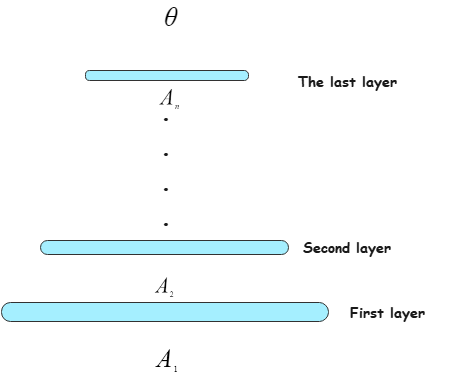
\includegraphics[width=4cm,height=4.0cm]{Figures/new.png}
	\end{figure}\\
	\par 求 $\dfrac{\mathrm{d} \theta}{\mathrm{d} A_{1}} $:
	\\\\由(\ref{con:inventoryflow2}) 可以知道:
	\begin{equation}
		\dfrac{\mathrm{d} \theta}{\mathrm{d} A_{1}}=\dfrac{\mathrm{d} A_{n}^{T}}{\mathrm{d} A_{1}} 
		\cdot
		\dfrac{\mathrm{d} \theta}{\mathrm{d} A_{n}}=(\dfrac{\mathrm{d} A_{n}}{\mathrm{d} A_{1}^{T}})^T
		\cdot
		\dfrac{\mathrm{d} \theta}{\mathrm{d} A_{n}}
	\end{equation}
	然后继续把$\dfrac{\mathrm{d} A_{n}}{\mathrm{d} A_{1}^{T}}$ 按照(\ref{con:inventoryflow3}) 展开:
	\begin{align*}
		\dfrac{\mathrm{d} A_{n}}{\mathrm{d} A_{1}^{T}}
		&=
		\dfrac{\mathrm{d} A_{n}}{\mathrm{d} A_{n-1}^{T}}
		\cdot
		\dfrac{\mathrm{d} A_{n-1}}{\mathrm{d} A_{1}^{T}}\\\\
		&=
		\dfrac{\mathrm{d} A_{n}}{\mathrm{d} A_{n-1}^{T}}
		\cdot
		\dfrac{\mathrm{d} A_{n-1}}{\mathrm{d} A_{n-2}^{T}}
		\cdot
		\dfrac{\mathrm{d} A_{n-2}}{\mathrm{d} A_{1}^{T}}\\\\
		&=
		\dfrac{\mathrm{d} A_{n}}{\mathrm{d} A_{n-1}^{T}}
		\cdot
		\dfrac{\mathrm{d} A_{n-1}}{\mathrm{d} A_{n-2}^{T}}
		\cdot
		\dfrac{\mathrm{d} A_{n-2}}{\mathrm{d} A_{n-3}^{T}}
		\cdot
		\dfrac{\mathrm{d} A_{n-3}}{\mathrm{d} A_{1}^{T}}\\\\
		&=
		\dfrac{\mathrm{d} A_{n}}{\mathrm{d} A_{n-1}^{T}}
		\cdot
		\dfrac{\mathrm{d} A_{n-1}}{\mathrm{d} A_{n-2}^{T}}
		\cdot
		\dfrac{\mathrm{d} A_{n-2}}{\mathrm{d} A_{n-3}^{T}}
		\cdot
		\dfrac{\mathrm{d} A_{n-3}}{\mathrm{d} A_{n-4}^{T}}
		\cdot
		\dfrac{\mathrm{d} A_{n-4}}{\mathrm{d} A_{1}^{T}}\\\\
		&=
		\dfrac{\mathrm{d} A_{n}}{\mathrm{d} A_{n-1}^{T}}
		\cdot
		\dfrac{\mathrm{d} A_{n-1}}{\mathrm{d} A_{n-2}^{T}}
		\cdot
		\dfrac{\mathrm{d} A_{n-2}}{\mathrm{d} A_{n-3}^{T}}
		\cdot
		\dfrac{\mathrm{d} A_{n-3}}{\mathrm{d} A_{n-4}^{T}}
		\cdot
		\dfrac{\mathrm{d} A_{n-4}}{\mathrm{d} A_{n-5}^{T}}
		\ldots \ldots
		\dfrac{\mathrm{d} A_{3}}{\mathrm{d} A_{2}^{T}}
		\cdot
		\dfrac{\mathrm{d} A_{2}}{\mathrm{d} A_{1}^{T}} 
	\end{align*}
	所以有:
	\begin{equation}
		\dfrac{\mathrm{d} \theta}{\mathrm{d} A_{1}}=(\dfrac{\mathrm{d} A_{n}}{\mathrm{d} A_{n-1}^{T}}
		\cdot
		\dfrac{\mathrm{d} A_{n-1}}{\mathrm{d} A_{n-2}^{T}}
		\cdot
		\dfrac{\mathrm{d} A_{n-2}}{\mathrm{d} A_{n-3}^{T}}
		\cdot
		\dfrac{\mathrm{d} A_{n-3}}{\mathrm{d} A_{n-4}^{T}}
		\cdot
		\dfrac{\mathrm{d} A_{n-4}}{\mathrm{d} A_{n-5}^{T}}
		\ldots \ldots
		\dfrac{\mathrm{d} A_{3}}{\mathrm{d} A_{2}^{T}}
		\cdot
		\dfrac{\mathrm{d} A_{2}}{\mathrm{d} A_{1}^{T}} )^T
		\cdot
		\dfrac{\mathrm{d} \theta}{\mathrm{d} A_{n}}
	\end{equation}
	\textbf{几种常用的推论:}\\
	\textbf{推论一 :}设:
	\begin{equation}
		A=\left[
		a_1,a_2,\ldots,a_m
		\right]_{1{\times}m} \quad X=\left[
			\begin{array}{c}
				x_1\\
				x_2\\
				\vdots
				x_m
			\end{array}
		\right]_{m{\times}1}
	\end{equation}
		求$\dfrac{\mathrm{d } (AX)}{\mathrm{d} X}$,$\dfrac{\mathrm{d } (AX)}{\mathrm{d} X^T}$:
		\begin{align}
			\dfrac{\mathrm{d } (AX)}{\mathrm{d} X}=\left[
				\begin{array}{c}
					\dfrac{\partial (AX)}{\partial x_1}\\\\
					\dfrac{\partial (AX)}{\partial x_2}\\\\
					\vdots\\\\
					\dfrac{\partial (AX)}{\partial x_m}\\		
				\end{array}
			\right]_{m{\times}1}
			=
			\left[
			\begin{array}{c}
				\dfrac{\partial \sum_{i=1}^{m}x_ia_i}{\partial x_1}\\\\
				\dfrac{\partial \sum_{i=1}^{m}x_ia_i}{\partial x_2}\\\\
				\vdots\\\\
				\dfrac{\partial \sum_{i=1}^{m}x_ia_i}{\partial x_m}\\		
			\end{array}
			\right]_{m{\times}1}
			=
			\left[
			\begin{array}{c}
				a_1\\
				a_2\\
				\vdots\\
				a_m		
			\end{array}
			\right]_{m{\times}1}=A
		\end{align}
	\begin{align}
		\dfrac{\mathrm{d } (AX)}{\mathrm{d} X^T}=\left[
		\begin{array}{cccc}
			\dfrac{\partial (AX)}{\partial x_1}&\dfrac{\partial (AX)}{\partial x_2}&\ldots&\dfrac{\partial (AX)}{\partial x_m}
		\end{array}
		\right]_{1{\times}m}=\left[
			\begin{array}{cccc}
				a_1 & a_2 & \ldots & a_m
			\end{array}
		\right]=A^T
	\end{align}
	\textbf{推论二 :}设:
	\begin{equation}
		A=\left[
		\begin{array}{cccc}
			a_{11}&a_{12}&\ldots&a_{1m}\\
			a_{21}&a_{22}&\ldots&a_{2m}\\
			\vdots&\vdots&\ddots&\vdots\\
			a_{n1}&a_{n2}&\ldots&a_{nm}
		\end{array}
		\right]_{n{\times}m} \quad X=\left[
		\begin{array}{c}
			x_1\\
			x_2\\
			\vdots
			x_m
		\end{array}
		\right]_{m{\times}1}
	\end{equation}
	求$\dfrac{\mathrm{d } (AX)}{\mathrm{d} X}$,$\dfrac{\mathrm{d } (AX)}{\mathrm{d} X^T}$:
	记:
	\begin{equation*}
		Y=AX=\left[
			\begin{array}{c}
				y_1\\
				y_2\\
				\vdots\\
				y_n
			\end{array}
		\right]  \quad\quad\text{且:}\quad\quad y_i=\sum_{k=1}^{m}a_{ik}x_k
	\end{equation*}
	\begin{align*}
		\dfrac{\mathrm{d } (AX)}{\mathrm{d} X}&=\left[
			\begin{array}{c}
				\dfrac{\partial Y}{\partial x_1}\\\\
				\dfrac{\partial Y}{\partial x_2}\\\\
				\vdots \\\\
				\dfrac{\partial Y}{\partial x_m}
			\end{array}
		\right]=
		\left[
		\begin{array}{cccc}
			\dfrac{\partial y_1}{\partial x_1} & \dfrac{\partial y_2}{\partial x_1} & \ldots&\dfrac{\partial y_n}{\partial x_1}\\\\
			\dfrac{\partial y_1}{\partial x_2} & \dfrac{\partial y_2}{\partial x_2} & \ldots&\dfrac{\partial y_n}{\partial x_2}\\\\
			\vdots & \vdots &\ddots & \vdots \\\\
			\dfrac{\partial y_1}{\partial x_m} & \dfrac{\partial y_2}{\partial x_m} & \ldots&\dfrac{\partial y_n}{\partial x_m}
		\end{array}
		\right]\\\\
		&=
		\left[
		\begin{array}{cccc}
			\dfrac{\partial \sum_{k=1}^{m}a_{1k}x_k}{\partial x_1} & \dfrac{\partial \sum_{k=1}^{m}a_{2k}x_k}{\partial x_1} & \ldots&\dfrac{\partial \sum_{k=1}^{m}a_{nk}x_k}{\partial x_1}\\\\
			\dfrac{\partial \sum_{k=1}^{m}a_{1k}x_k}{\partial x_2} & \dfrac{\partial \sum_{k=1}^{m}a_{2k}x_k}{\partial x_2} & \ldots&\dfrac{\partial \sum_{k=1}^{m}a_{nk}x_k}{\partial x_2}\\\\
			\vdots & \vdots &\ddots & \vdots \\\\
			\dfrac{\partial \sum_{k=1}^{m}a_{1k}x_k}{\partial x_m} & \dfrac{\partial \sum_{k=1}^{m}a_{2k}x_k}{\partial x_m} & \ldots&\dfrac{\partial \sum_{k=1}^{m}a_{nk}x_k}{\partial x_m}
		\end{array}
		\right]\\\\
		&=\left[
			\begin{array}{cccc}
				a_{11} & a_{21} & \ldots & a_{n1}\\
				a_{12} & a_{22} & \ldots & a_{n2}\\
				\vdots & \vdots &\ddots & \vdots\\
				a_{1m} & a_{2m} & \ldots & a_{nm}\\
			\end{array}
		\right]=A^T
	\end{align*}
	同理可得:
	\begin{equation}
			\dfrac{\mathrm{d } (AX)}{\mathrm{d} X^T}=A
	\end{equation}
	\par \textbf{设:}
	\begin{equation*}
		X=\left[
			x_1,x_2,x_3,......,x_n
		\right]^T_{n{\times}1}
	\end{equation*}
	求$\dfrac{\mathrm{d} \Vert X \Vert}{\mathrm{d} X}$,$\dfrac{\mathrm{d} \Vert X \Vert}{\mathrm{d} X^T}$:
	\begin{equation}
		\dfrac{\mathrm{d} \Vert X \Vert}{\mathrm{d} X}
		=
		\left[
			\begin{array}{c}
				\dfrac{\mathrm{d} \Vert X \Vert}{\mathrm{d} x_1}\\\\
				\dfrac{\mathrm{d} \Vert X \Vert}{\mathrm{d} x_2}\\\\
				\vdots\\\\
				\dfrac{\mathrm{d} \Vert X \Vert}{\mathrm{d} x_n}
			\end{array}
		\right]
		=
		\left[
		\begin{array}{c}
			\dfrac{\mathrm{d} \sum_{i=1}^{n} x_i^2}{\mathrm{d} x_1}\\\\
			\dfrac{\mathrm{d} \sum_{i=1}^{n} x_i^2}{\mathrm{d} x_2}\\\\
			\vdots\\\\
			\dfrac{\mathrm{d} \sum_{i=1}^{n} x_i^2}{\mathrm{d} x_n}
		\end{array}
		\right]
		=
		\left[
		\begin{array}{c}
			2x_1\\
			2x_2\\
			\vdots\\
			2x_n
		\end{array}
		\right]
		=
		2X
	\end{equation}
	\begin{equation}
		\dfrac{\mathrm{d} \Vert X \Vert}{\mathrm{d} X^T}
		=
		\left[
		\begin{array}{c}
			\dfrac{\mathrm{d} \Vert X \Vert}{\mathrm{d} x_1}\\\\
			\dfrac{\mathrm{d} \Vert X \Vert}{\mathrm{d} x_2}\\\\
			\vdots\\\\
			\dfrac{\mathrm{d} \Vert X \Vert}{\mathrm{d} x_n}
		\end{array}
		\right]^T
		=
		\left[
		\begin{array}{c}
			\dfrac{\mathrm{d} \sum_{i=1}^{n} x_i^2}{\mathrm{d} x_1}\\\\
			\dfrac{\mathrm{d} \sum_{i=1}^{n} x_i^2}{\mathrm{d} x_2}\\\\
			\vdots\\\\
			\dfrac{\mathrm{d} \sum_{i=1}^{n} x_i^2}{\mathrm{d} x_n}
		\end{array}
		\right]^T
		=
		\left[
		\begin{array}{c}
			2x_1\\
			2x_2\\
			\vdots\\
			2x_n
		\end{array}
		\right]^T
		=
		2X^T
	\end{equation}


	
	



	
	 

	
	
	


	
	
	


	
	
	
	
	
\end{document}
	

